\documentclass[a4paper,12pt]{article} 
\usepackage[T2A]{fontenc}			
\usepackage[utf8]{inputenc}			
\usepackage[english,russian]{babel}	
\usepackage{amsmath,amsfonts,amssymb,amsthm,mathtools} 
\usepackage[colorlinks, linkcolor = blue]{hyperref}
\usepackage{upgreek}\usepackage[left=2cm,right=2cm,top=2cm,bottom=3cm,bindingoffset=0cm]{geometry}
\usepackage{multirow}
\usepackage{graphicx}
\usepackage{xcolor}
\author{Дорогинин Д.В.}
\title{3.2.2. Резонанс напряжений.}
\date{\today}
\begin{document}
\maketitle
\newpage
\textbf{Цель работы}: исследование резонанса напряжений в последовательном колебательном контуре с изменяемой ёмкостью, включающее получение амплитудно-частотных и фазово-частотных характеристик, а также определение основных параметров контура.


\textbf{В работе используются}: генератор сигналов, источник напряжения, нагруженный на последовательный колебательный контур с переменной ёмкостью, двулучевой осциллограф, цифровые вольтметры.
\section*{Описание работы}
\begin{center}
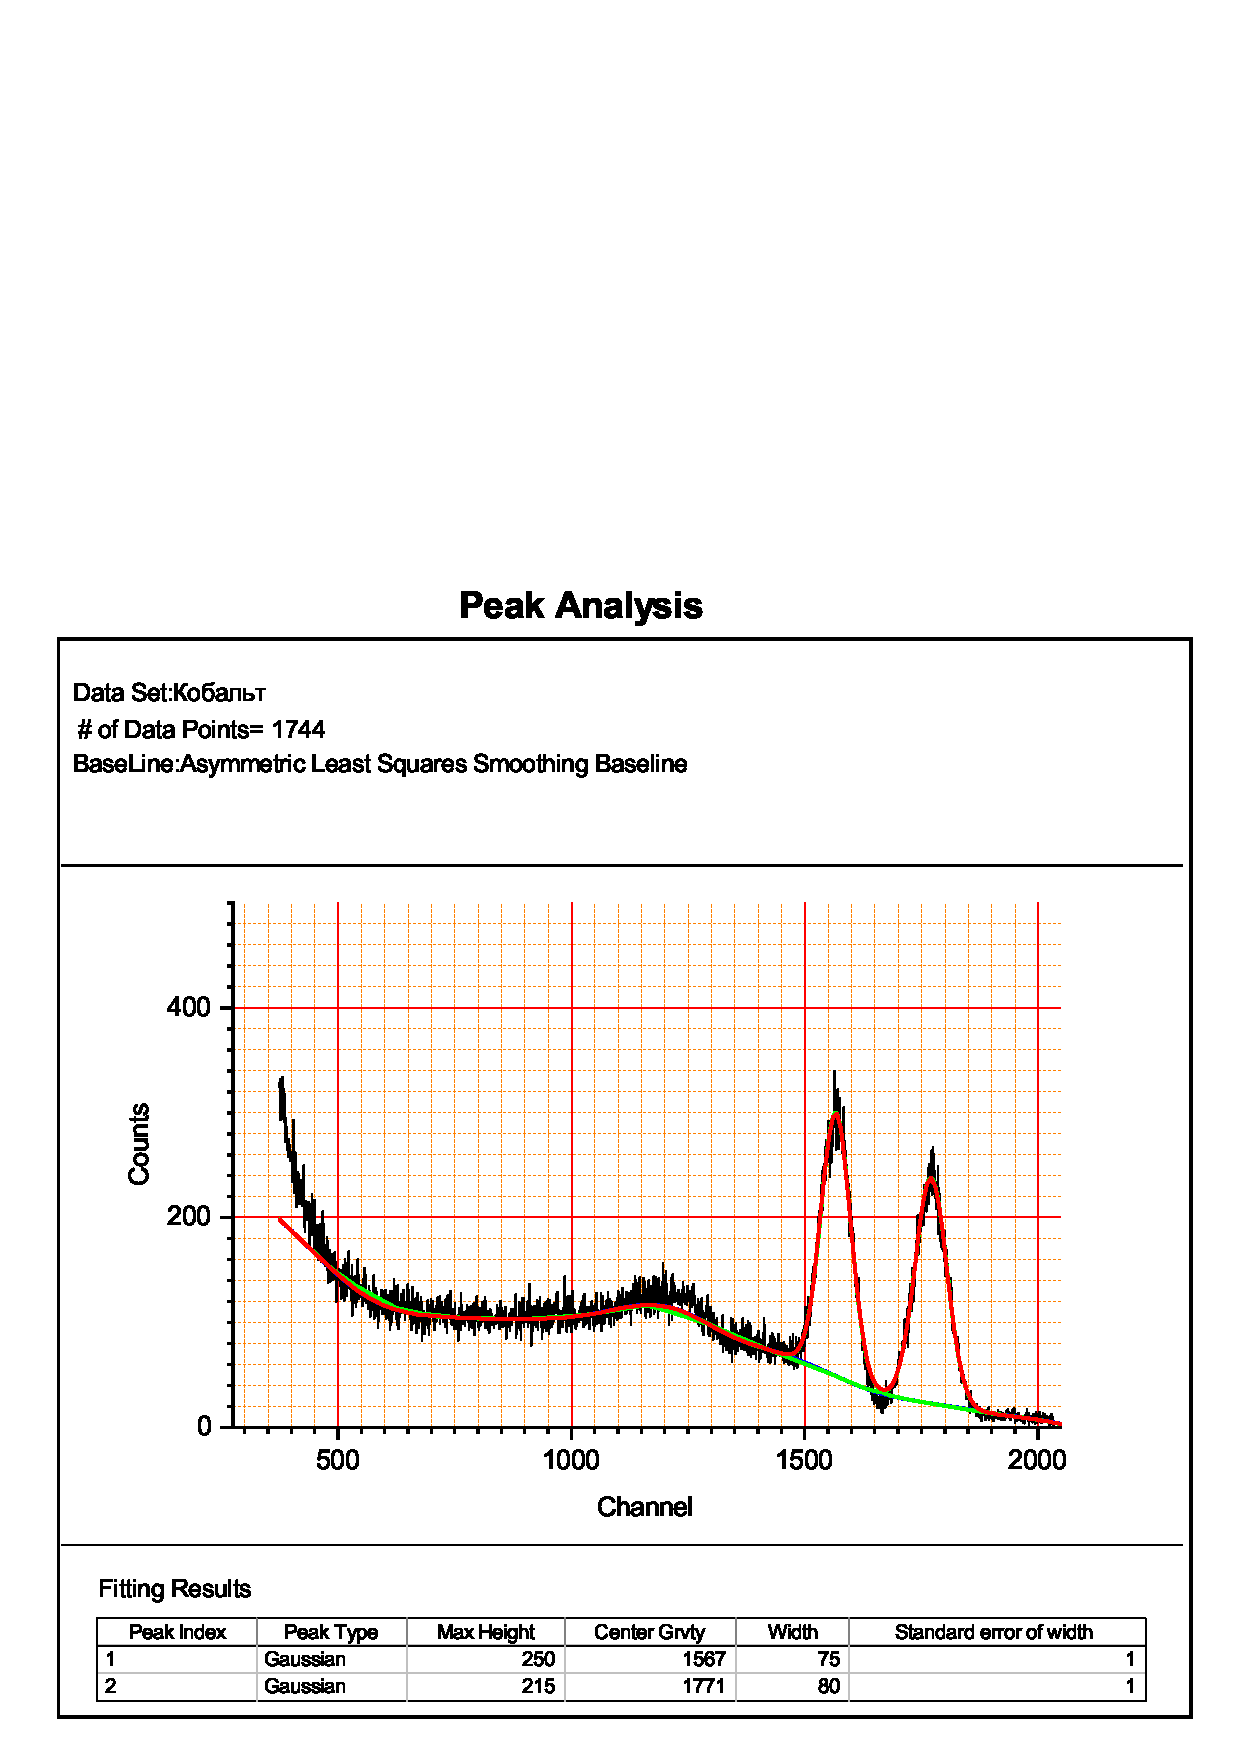
\includegraphics[width = 0.5\textwidth]{2.png}
\end{center}
Схема экспериментального стенда для изучения резонанса напряжений в последовательном колебательном контуре показана на рисунке. Синусоидальный сигнал от генератора GFG8255A поступает через согласующую RC-цепочку на вход источника напряжения, собранного на операционном усилителе ОУ. Питание операционного усилителя осуществляется
встроенным блоком-выпрямителем от сети переменного тока 220 Вольт (цепь питания на
схеме не показана). Источник напряжения, обладающий по определению нулевым внутренним сопротивлением, фактически обеспечивает с высокой точностью постоянство амплитуды сигнала на меняющейся по величине нагрузке – последовательном колебательном контуре, изображенном на рисунке в виде эквивалентной схемы.
\section*{Ход работы}
\begin{enumerate}
\item Подготавливаем установку к работе и включаем приборы.
\item Выставляем на входе контура напряжение $E = 100~\text{мВ}$, в течении всей работы поддерживая его постоянным.
\item Добиваемся получения двух отцентрованных синусоид на осциллографе. Убеждаемся, что одна из синусоид при изменении частоты $f$ генератора меняет амплитуду относительно начала координа, в то время как амплитуда другой не меняется с погрешностью не более 1\%.
\item Для контуров с семью различными ёмкостями, меняя их с помощью переключателя на
блоке, измеряем резонансные частоты $f_{0n}$ и напряжения $U_C(f_{0n})$. Регистрируйем также
напряжения $E(f_{0n})$, игнорируя отклонения в пределах относительной погрешности 1%.
\item Для контуров ёмкостями $C_1 = 25~\text{нФ}$ и $C_1 = 57.2~\text{нФ}$ снимаем амплитудно-частотные характеристики $U_C(f)$ (16-17 точек
в сумме по обе стороны от резонанса) при том же напряжении $E$.
\begin{table}[h]
\centering
\begin{tabular}{ccccc||c|c|c|c|c|}
\hline
\multicolumn{5}{|c||}{$C_1 = 25,0$ нФ}                                                                                                         & \multicolumn{5}{c|}{$C_4 = 57,2$ нФ}        \\ \hline
\multicolumn{1}{|c|}{$n$} & \multicolumn{1}{c|}{$f$, кГц} & \multicolumn{1}{c|}{$\sigma_f$, кГц} & \multicolumn{1}{c|}{$A$, В} & $\sigma_A$, В         & $n$ & f, кГц & $\sigma_f$, кГц & A, В & $\sigma_A$, В \\ \hline
\multicolumn{1}{|c|}{1}   & \multicolumn{1}{c|}{29,8}     & \multicolumn{1}{c|}{0,1}             & \multicolumn{1}{c|}{0,40}   & 0,01                  & 1   & 17     & 0,1             & 0,13 & 0,01          \\ \hline
\multicolumn{1}{|c|}{2}   & \multicolumn{1}{c|}{27,3}     & \multicolumn{1}{c|}{0,1}             & \multicolumn{1}{c|}{0,20}   & 0,01                  & 2   & 17,6   & 0,1             & 0,18 & 0,01          \\ \hline
\multicolumn{1}{|c|}{3}   & \multicolumn{1}{c|}{28}       & \multicolumn{1}{c|}{0,1}             & \multicolumn{1}{c|}{0,22}   & 0,01                  & 3   & 18,4   & 0,1             & 0,22 & 0,01          \\ \hline
\multicolumn{1}{|c|}{4}   & \multicolumn{1}{c|}{28,5}     & \multicolumn{1}{c|}{0,1}             & \multicolumn{1}{c|}{0,25}   & 0,01                  & 4   & 18,7   & 0,1             & 0,24 & 0,01          \\ \hline
\multicolumn{1}{|c|}{5}   & \multicolumn{1}{c|}{29}       & \multicolumn{1}{c|}{0,1}             & \multicolumn{1}{c|}{0,28}   & 0,01                  & 5   & 19     & 0,1             & 0,26 & 0,01          \\ \hline
\multicolumn{1}{|c|}{6}   & \multicolumn{1}{c|}{29,5}     & \multicolumn{1}{c|}{0,1}             & \multicolumn{1}{c|}{0,32}   & 0,01                  & 6   & 19,3   & 0,1             & 0,30 & 0,01          \\ \hline
\multicolumn{1}{|c|}{7}   & \multicolumn{1}{c|}{30,5}     & \multicolumn{1}{c|}{0,1}             & \multicolumn{1}{c|}{0,48}   & 0,01                  & 7   & 19,5   & 0,1             & 0,32 & 0,01          \\ \hline
\multicolumn{1}{|c|}{8}   & \multicolumn{1}{c|}{30,9}     & \multicolumn{1}{c|}{0,1}             & \multicolumn{1}{c|}{0,60}   & 0,01                  & 8   & 19,7   & 0,1             & 0,34 & 0,01          \\ \hline
\multicolumn{1}{|c|}{9}   & \multicolumn{1}{c|}{31,3}     & \multicolumn{1}{c|}{0,1}             & \multicolumn{1}{c|}{0,90}   & 0,01                  & 9   & 20     & 0,1             & 0,4  & 0,01          \\ \hline
\multicolumn{1}{|c|}{10}  & \multicolumn{1}{c|}{31,5}     & \multicolumn{1}{c|}{0,1}             & \multicolumn{1}{c|}{1,00}   & 0,01                  & 10  & 20,2   & 0,1             & 0,48 & 0,01          \\ \hline
\multicolumn{1}{|c|}{11}  & \multicolumn{1}{c|}{31,7}     & \multicolumn{1}{c|}{0,1}             & \multicolumn{1}{c|}{1,10}   & 0,01                  & 11  & 20,3   & 0,1             & 0,52 & 0,01          \\ \hline
\multicolumn{1}{|c|}{12}  & \multicolumn{1}{c|}{31,9}     & \multicolumn{1}{c|}{0,1}             & \multicolumn{1}{c|}{1,30}   & 0,01                  & 12  & 20,5   & 0,1             & 0,6  & 0,01          \\ \hline
\multicolumn{1}{|c|}{13}  & \multicolumn{1}{c|}{32}       & \multicolumn{1}{c|}{0,1}             & \multicolumn{1}{c|}{1,40}   & 0,01                  & 13  & 20,7   & 0,1             & 0,78 & 0,01          \\ \hline
\multicolumn{1}{|c|}{14}  & \multicolumn{1}{c|}{32,2}     & \multicolumn{1}{c|}{0,1}             & \multicolumn{1}{c|}{1,35}   & 0,01                  & 14  & 20,8   & 0,1             & 0,83 & 0,01          \\ \hline
\multicolumn{1}{|c|}{15}  & \multicolumn{1}{c|}{32,4}     & \multicolumn{1}{c|}{0,1}             & \multicolumn{1}{c|}{1,25}   & 0,01                  & 15  & 21,1   & 0,1             & 1,00 & 0,01          \\ \hline
\multicolumn{1}{|c|}{16}  & \multicolumn{1}{c|}{32,8}     & \multicolumn{1}{c|}{0,1}             & \multicolumn{1}{c|}{0,90}   & 0,01                  & 16  & 21,2   & 0,1             & 1,00 & 0,01          \\ \hline
\multicolumn{1}{|c|}{17}  & \multicolumn{1}{c|}{33,1}     & \multicolumn{1}{c|}{0,1}             & \multicolumn{1}{c|}{0,75}   & 0,01                  & 17  & 21,4   & 0,1             & 1,00 & 0,01          \\ \hline
\multicolumn{1}{|c|}{18}  & \multicolumn{1}{c|}{33,6}     & \multicolumn{1}{c|}{0,1}             & \multicolumn{1}{c|}{0,60}   & 0,01                  & 18  & 21,6   & 0,1             & 0,80 & 0,01          \\ \hline
\multicolumn{1}{|c|}{19}  & \multicolumn{1}{c|}{34,1}     & \multicolumn{1}{c|}{0,1}             & \multicolumn{1}{c|}{0,40}   & 0,01                  & 19  & 21,8   & 0,1             & 0,72 & 0,01          \\ \hline
\multicolumn{1}{|c|}{20}  & \multicolumn{1}{c|}{34,6}     & \multicolumn{1}{c|}{0,1}             & \multicolumn{1}{c|}{0,35}   & 0,01                  & 20  & 21,9   & 0,1             & 0,64 & 0,01          \\ \hline
\multicolumn{1}{|c|}{21}  & \multicolumn{1}{c|}{35,1}     & \multicolumn{1}{c|}{0,1}             & \multicolumn{1}{c|}{0,24}   & 0,01                  & 21  & 22,1   & 0,1             & 0,54 & 0,01          \\ \hline
\multicolumn{1}{|c|}{22}  & \multicolumn{1}{c|}{35,4}     & \multicolumn{1}{c|}{0,1}             & \multicolumn{1}{c|}{0,24}   & 0,01                  & 22  & 22,6   & 0,1             & 0,4  & 0,01          \\ \hline
\multicolumn{1}{|c|}{23}  & \multicolumn{1}{c|}{36,6}     & \multicolumn{1}{c|}{0,1}             & \multicolumn{1}{c|}{0,18}   & 0,01                  & 23  & 22,9   & 0,1             & 0,32 & 0,01          \\ \hline
\multicolumn{1}{|c|}{24}  & \multicolumn{1}{c|}{37,3}     & \multicolumn{1}{c|}{0,1}             & \multicolumn{1}{c|}{0,16}   & 0,01                  & 24  & 23,2   & 0,1             & 0,28 & 0,01          \\ \hline
\multicolumn{1}{|c|}{25}  & \multicolumn{1}{c|}{32,5}     & \multicolumn{1}{c|}{0,1}             & \multicolumn{1}{c|}{1,30}   & 0,01                  & 25  & 23,6   & 0,1             & 0,24 & 0,01          \\ \hline
\multicolumn{1}{|c|}{26}  & \multicolumn{1}{c|}{32,9}     & \multicolumn{1}{c|}{0,1}             & \multicolumn{1}{c|}{0,85}   & 0,01                  & 26  & 23,8   & 0,1             & 0,22 & 0,01          \\ \hline
\multicolumn{1}{|c|}{27}  & \multicolumn{1}{c|}{33}       & \multicolumn{1}{c|}{0,1}             & \multicolumn{1}{c|}{0,80}   & 0,01                  & 27  & 24,3   & 0,1             & 0,18 & 0,01          \\ \hline
\multicolumn{1}{l}{}      & \multicolumn{1}{l}{}          & \multicolumn{1}{l}{}                 & \multicolumn{1}{l}{}        & \multicolumn{1}{l|}{} & 28  & 24,6   & 0,1             & 0,16 & 0,01          \\ \cline{6-10} 
\multicolumn{1}{l}{}      & \multicolumn{1}{l}{}          & \multicolumn{1}{l}{}                 & \multicolumn{1}{l}{}        & \multicolumn{1}{l|}{} & 29  & 24,9   & 0,1             & 0,15 & 0,01          \\ \cline{6-10} 
\end{tabular}
\end{table}
\newpage
\item Для тех же двух контуров снимите фазово-частотные характеристики $\varphi_C(f)$ (16-17 точек в сумме по обе стороны от резонанса) при том же
напряжении $E$.
\begin{table}[h]
\centering
\begin{tabular}{ccc||c|c|c|}
\hline
\multicolumn{3}{|c||}{$C_1 = 25,0 $ нФ} & \multicolumn{3}{c|}{$C_4 = 57,2$ нФ} \\ \hline
\multicolumn{1}{|c|}{$n$} & \multicolumn{1}{c|}{$f$, кГц} & $-\varphi/ \pi$ & $n$ & $f$, кГц & $-\varphi/ \pi$ \\ \hline
\multicolumn{1}{|c|}{1} & \multicolumn{1}{c|}{29,6} & 0,03 & 1 & 18,8 & 0,06 \\ \hline
\multicolumn{1}{|c|}{2} & \multicolumn{1}{c|}{29,8} & 0,04 & 2 & 19 & 0,08 \\ \hline
\multicolumn{1}{|c|}{3} & \multicolumn{1}{c|}{30} & 0,05 & 3 & 19,5 & 0,08 \\ \hline
\multicolumn{1}{|c|}{4} & \multicolumn{1}{c|}{30,4} & 0,05 & 4 & 19,6 & 0,11 \\ \hline
\multicolumn{1}{|c|}{5} & \multicolumn{1}{c|}{30,8} & 0,1 & 5 & 19,8 & 0,15 \\ \hline
\multicolumn{1}{|c|}{6} & \multicolumn{1}{c|}{31,2} & 0,14 & 6 & 20,1 & 0,17 \\ \hline
\multicolumn{1}{|c|}{7} & \multicolumn{1}{c|}{31,5} & 0,21 & 7 & 20,3 & 0,2 \\ \hline
\multicolumn{1}{|c|}{8} & \multicolumn{1}{c|}{31,6} & 0,29 & 8 & 20,5 & 0,22 \\ \hline
\multicolumn{1}{|c|}{9} & \multicolumn{1}{c|}{31,9} & 0,4 & 9 & 20,7 & 0,27 \\ \hline
\multicolumn{1}{|c|}{10} & \multicolumn{1}{c|}{32} & 0,49 & 10 & 20,8 & 0,36 \\ \hline
\multicolumn{1}{|c|}{11} & \multicolumn{1}{c|}{32,3} & 0,6 & 11 & 21 & 0,41 \\ \hline
\multicolumn{1}{|c|}{12} & \multicolumn{1}{c|}{32,5} & 0,71 & 12 & 21,1 & 0,45 \\ \hline
\multicolumn{1}{|c|}{13} & \multicolumn{1}{c|}{32,8} & 0,8 & 13 & 21,2 & 0,48 \\ \hline
\multicolumn{1}{|c|}{14} & \multicolumn{1}{c|}{33} & 0,86 & 14 & 21,3 & 0,57 \\ \hline
\multicolumn{1}{|c|}{15} & \multicolumn{1}{c|}{33,2} & 0,87 & 15 & 21,5 & 0,71 \\ \hline
\multicolumn{1}{|c|}{16} & \multicolumn{1}{c|}{33,5} & 0,88 & 16 & 21,7 & 0,81 \\ \hline
\multicolumn{1}{|c|}{17} & \multicolumn{1}{c|}{33,8} & 0,94 & 17 & 22 & 0,86 \\ \hline
\multicolumn{1}{|c|}{18} & \multicolumn{1}{c|}{34} & 0,98 & 18 & 22,3 & 0,93 \\ \hline
\multicolumn{1}{|c|}{19} & \multicolumn{1}{c|}{34,4} & 1 & 19 & 22,4 & 1 \\ \hline
\multicolumn{1}{|c|}{20} & \multicolumn{1}{c|}{32,6} & 0,74 & 20 & 22,6 & 1,11 \\ \hline
\multicolumn{1}{|c|}{21} & \multicolumn{1}{c|}{32,4} & 0,66 & 21 & 22,8 & 1 \\ \hline
 &  &  & 22 & 23,1 & 0,98 \\ \cline{4-6} 
\end{tabular}
\end{table}
\end{enumerate}
\newpage
\section*{Обработка данных}
\begin{enumerate}
\item Результаты измерений представим в таблице.\\
\begin{table}[h]
\centering
\begin{tabular}{|c|c|c|c|c|c|c|c|c|c|c|c|}
\hline
$n$ & $C_n$, нФ & \begin{tabular}[c]{@{}c@{}}$f_{0n}$, \\ кГц\end{tabular} & $U_C$, В & $E$, В & \begin{tabular}[c]{@{}c@{}}$L$, \\ мкГн\end{tabular} & $Q$ & \begin{tabular}[c]{@{}c@{}}$\rho$, \\ Ом\end{tabular} & \begin{tabular}[c]{@{}c@{}}$R_{\sum}$, \\ Ом\end{tabular} & \begin{tabular}[c]{@{}c@{}}$R_{S_{\max}}$,\\ Ом\end{tabular} & $R_L$, Ом & $I$, мА \\ \hline
1 & 25,0 & 32,0 & 2,57 & 0,1 & 991,43 & 25 & 199,14 & 12,55 & 0,20 & 8,90 & 0,0080 \\ \hline
2 & 33,2 & 28,0 & 2,14 & 0,1 & 975,10 & 25 & 171,38 & 10,80 & 0,17 & 7,18 & 0,0093 \\ \hline
3 & 47,5 & 23,3 & 1,98 & 0,1 & 984,23 & 25 & 143,95 & 9,07 & 0,14 & 5,47 & 0,0110 \\ \hline
4 & 57,2 & 21,2 & 1,83 & 0,1 & 987,27 & 25 & 131,38 & 8,28 & 0,13 & 4,70 & 0,0121 \\ \hline
5 & 67,4 & 19,6 & 1,70 & 0,1 & 980,24 & 25 & 120,60 & 7,60 & 0,12 & 4,03 & 0,0132 \\ \hline
6 & 82,1 & 17,7 & 1,57 & 0,1 & 986,77 & 25 & 109,63 & 6,91 & 0,11 & 3,35 & 0,0145 \\ \hline
7 & 99,6 & 16,2 & 1,44 & 0,1 & 970,99 & 25 & 98,74 & 6,22 & 0,10 & 2,67 & 0,0161 \\ \hline
\multicolumn{5}{|c|}{Среднее значение} & 982,29 & \multicolumn{4}{c|}{--} & 5,18 & -- \\ \hline
\multicolumn{5}{|c|}{\begin{tabular}[c]{@{}c@{}}Среднеквадратичная погрешность\\ среднего значения\end{tabular}} & 2,74 & \multicolumn{4}{c|}{--} & 0,83 & -- \\ \hline
\multicolumn{5}{|c|}{\begin{tabular}[c]{@{}c@{}}Коэффициент Стьюденса\\ $t_{n \alpha}$ для\\ $n = 7$, $\alpha = 0,95$\end{tabular}} & 2,34 & \multicolumn{4}{c|}{--} & 2,34 & -- \\ \hline
\multicolumn{5}{|c|}{Случайная погрешность} & 6,42 & \multicolumn{4}{c|}{--} & 1,95 & -- \\ \hline
\end{tabular}
\end{table}
\item По данным из пункта 5 построим на одном графике амплитудо-частотные характеристики в координатах $f, U_C(f)$.\begin{center}
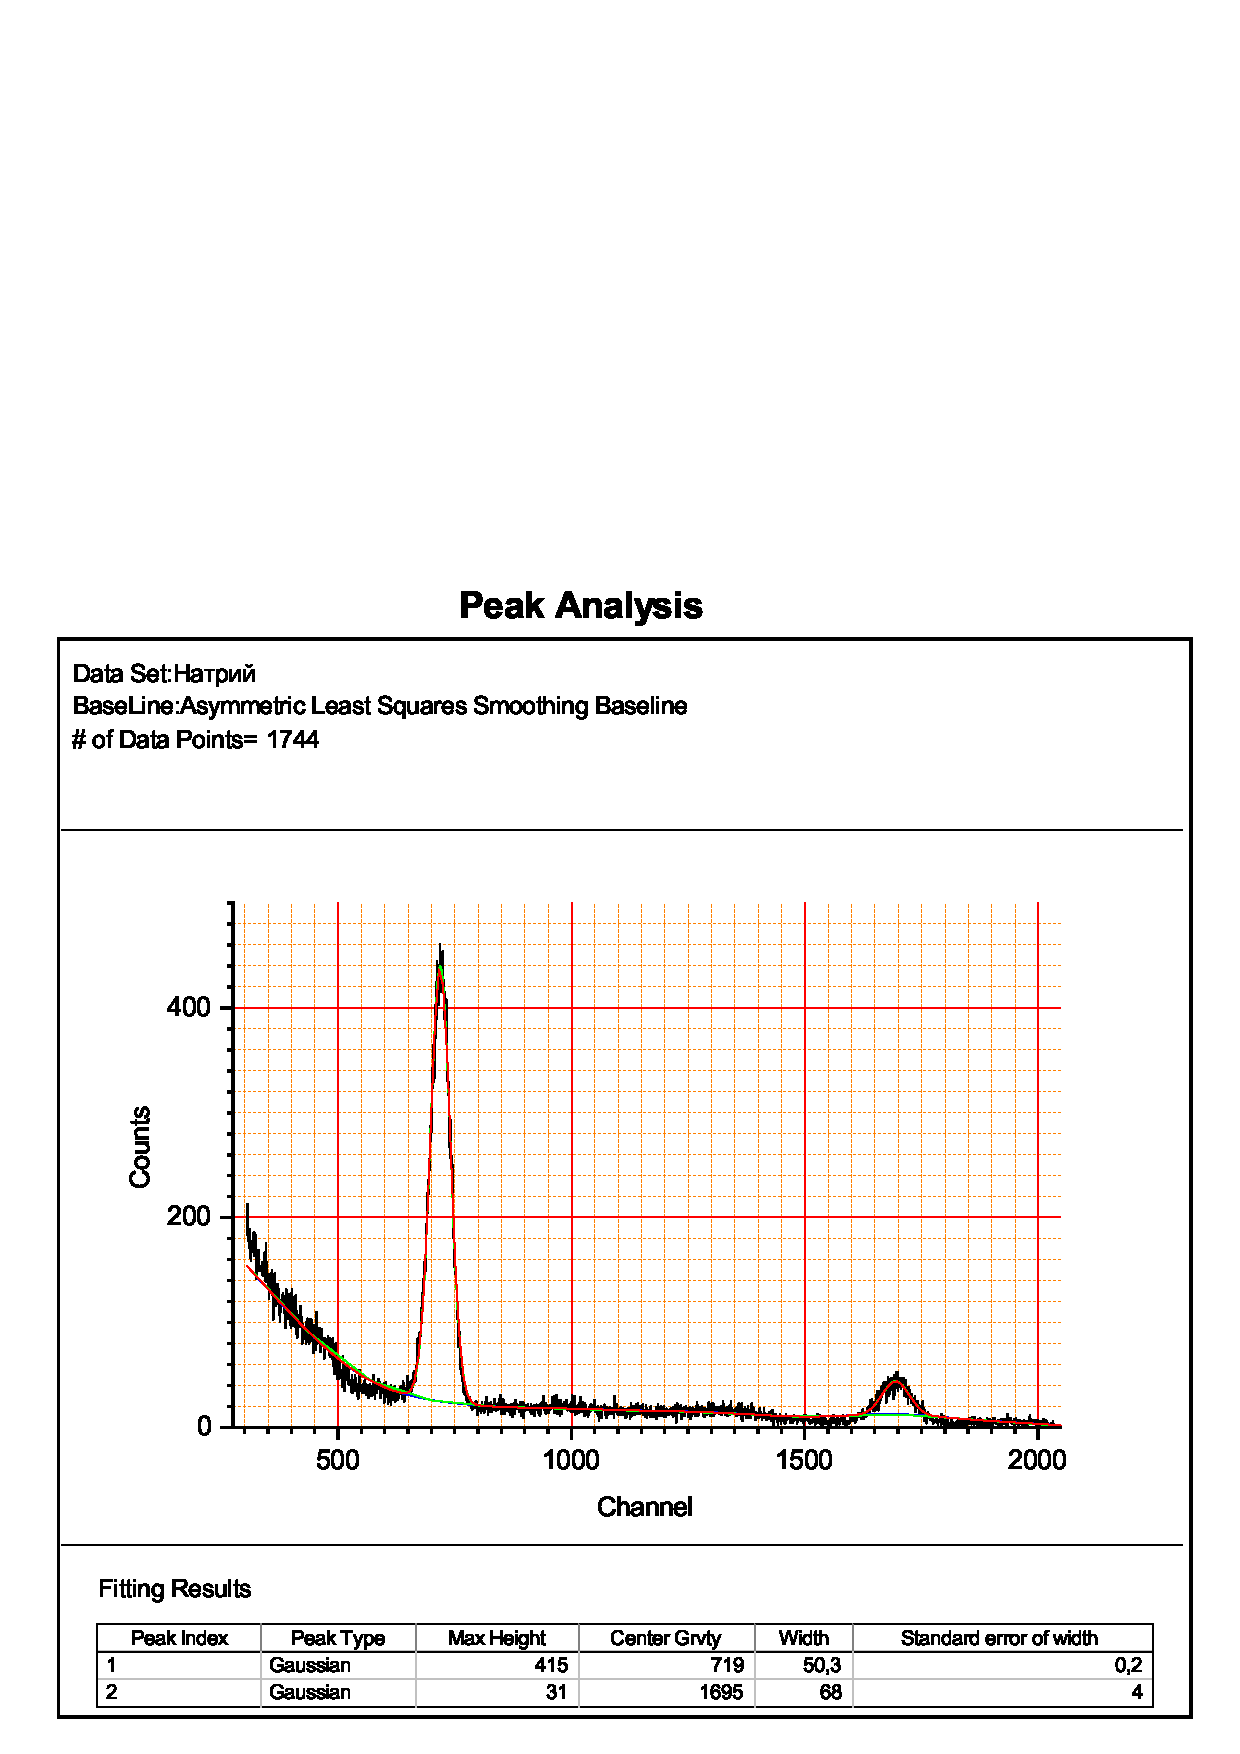
\includegraphics[width = 0.65\textwidth]{1.png}
\end{center}
\item По тем же данным построим на одном графике амплитудо-частотные характеристики в безразмерных координатах $x = f/f_{0n}, y = U_C(x)/U_C(1)$. По ширине резонансных кривых на уровне $0.707$ определим добротности $Q$ соответствующих контуров: $Q_1 = 25 \pm 5$ и $Q_2 = 22 \pm 4$.
\begin{center}
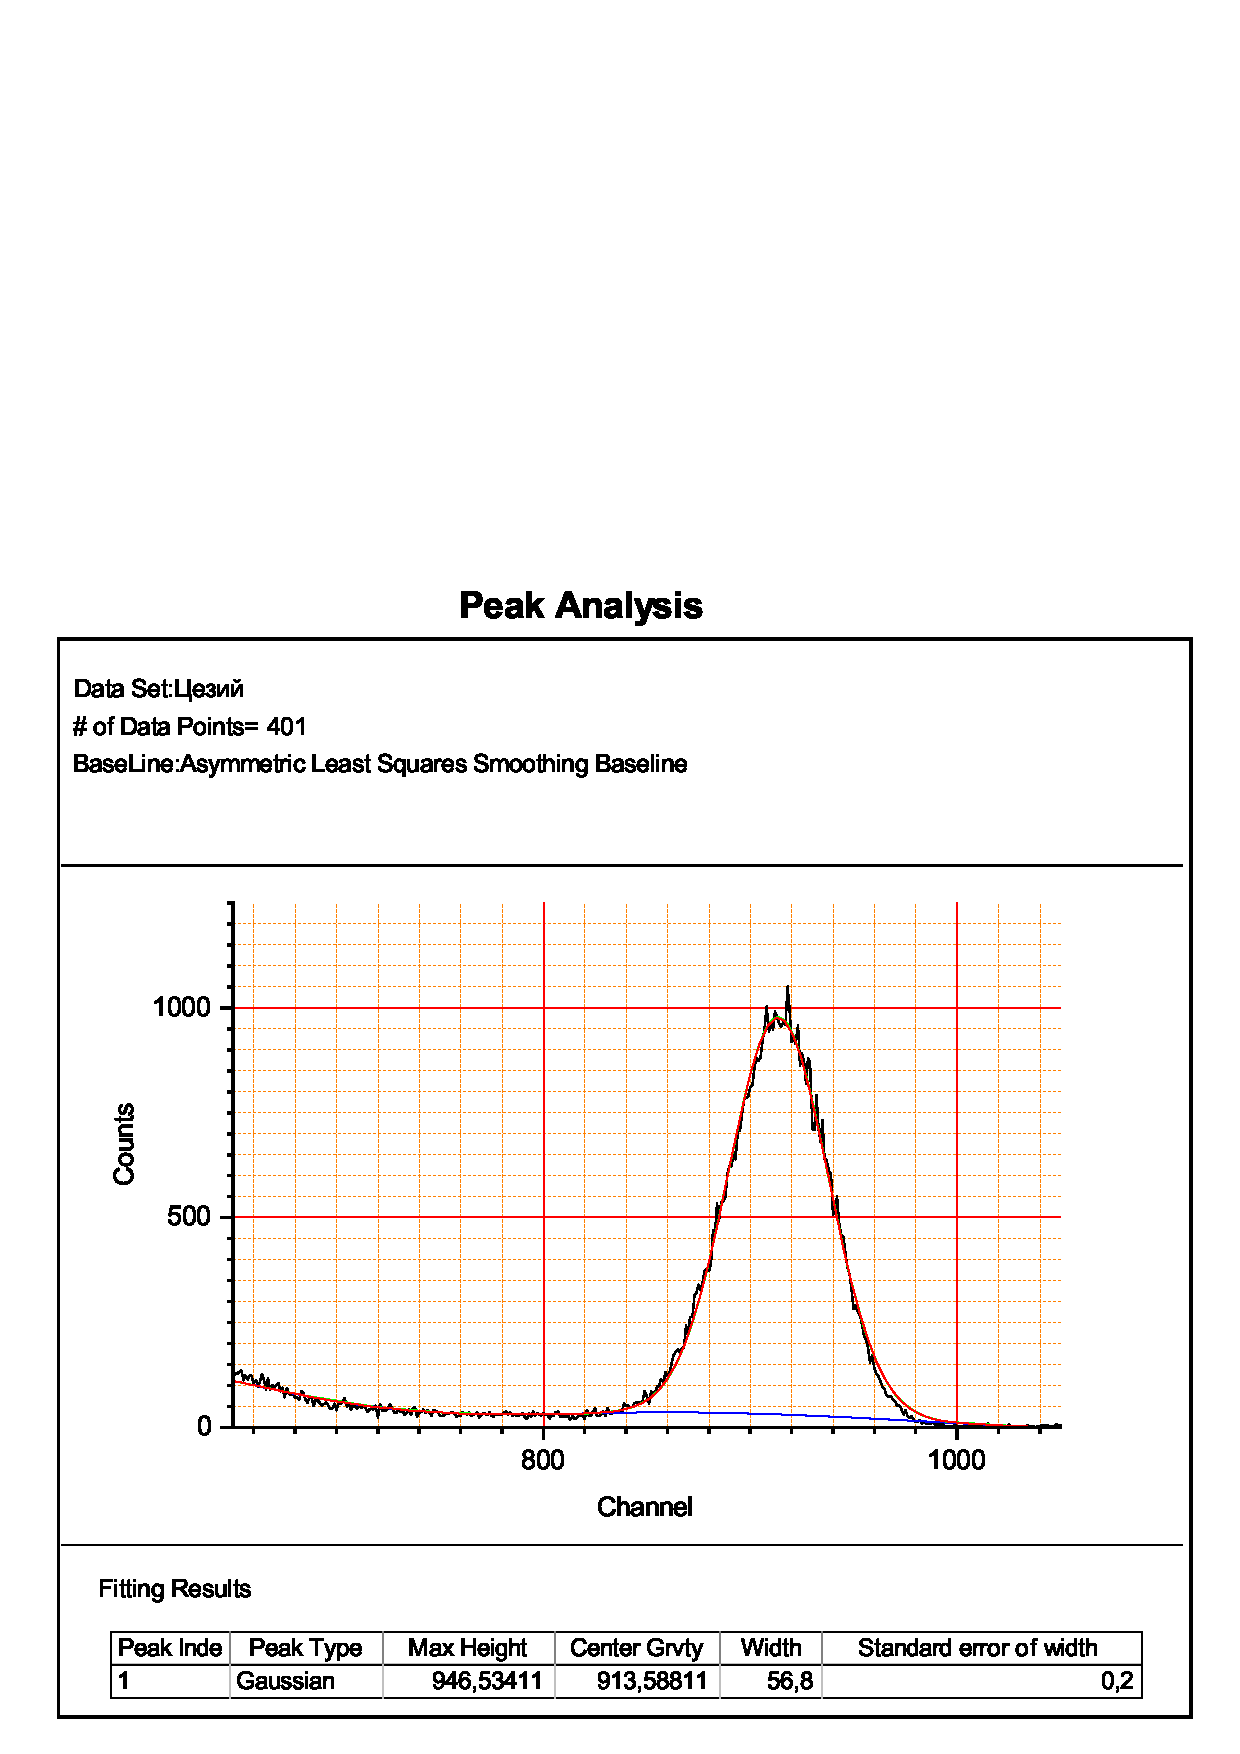
\includegraphics[width = 0.65\textwidth]{3.png}
\end{center}
\item По данным пункта 6 построим на одном графике фазово-частотные характеристики в координатах $x = f/f_{0n}, y = \varphi /\pi$ для выбранных контуров. По этим характеристикам определим добротности контуров одним из двух способов: по расстоянию между
точками по оси $x$, в которых $y$ меняется от $-0.25$ до $-0.75$, равному $1/Q$, или по формуле $Q = 0.5~d\varphi_C(x)/dx$ при $x=0$: $Q_1 = 25 \pm 4$ и $Q_2 = 33 \pm 5$.
\begin{center}
\includegraphics[width = 0.65\textwidth]{4.png}
\end{center}
\item По данным таблицы построим зависимость $R_L(f_{0n})$, на график нанесём прямую $\langle R_L \rangle$.
\begin{center}
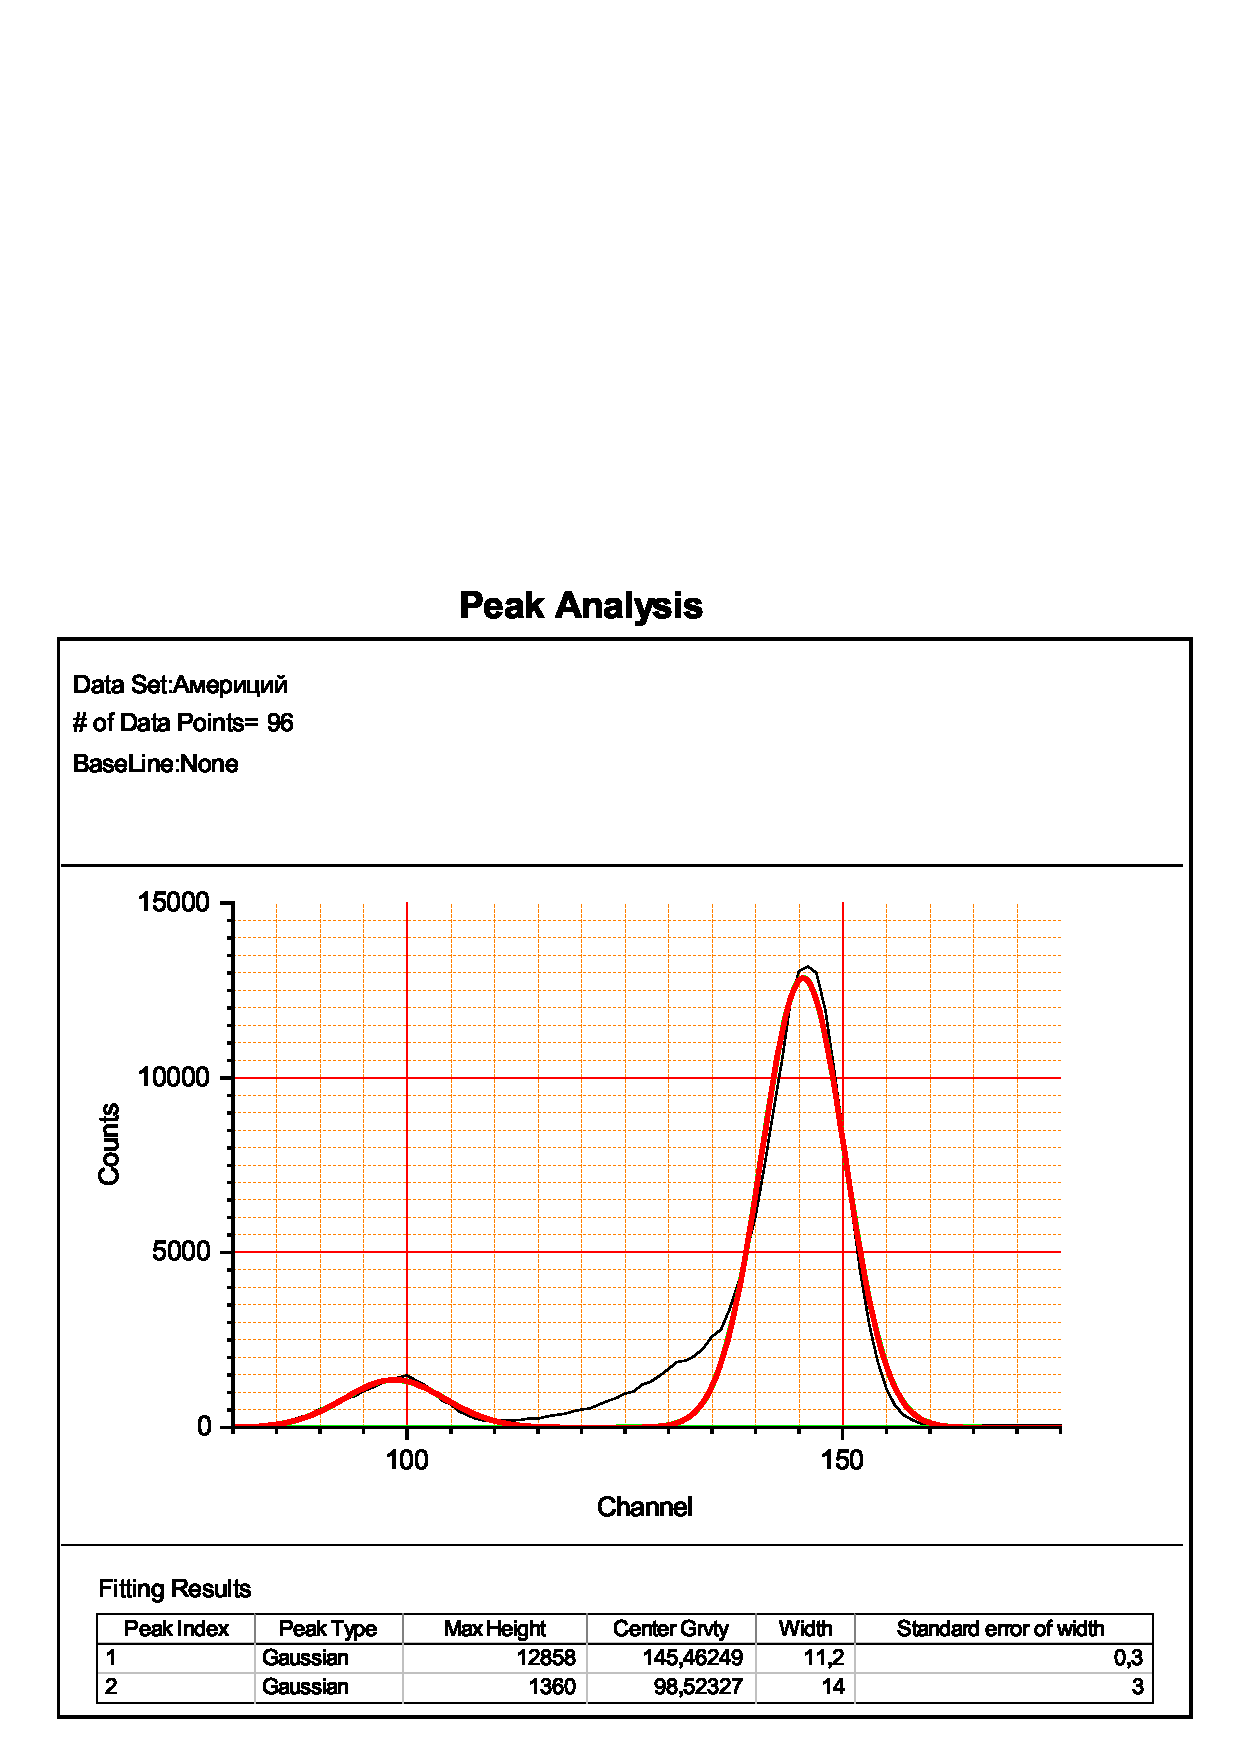
\includegraphics[width = 0.6\textwidth]{5.png}
\end{center}
\item По данным построим векторную диаграмму тока
и напряжений для контура с наименьшей добротностью в резонансном состоянии. Ось
абсцисс направим по вектору $\vec{E}$. Масштаб по этой оси сделаем в 2 раза более крупным,
чем по оси ординат.
\end{enumerate}
\end{document}